\documentclass{article}
\usepackage{xeCJK} 
\usepackage{amsmath}
\usepackage{amsfonts}
\usepackage{amssymb}
\usepackage{graphicx} 
\usepackage{tikz}
\usepackage{caption}

\setCJKmainfont{SimSun}[BoldFont=SimHei]

\usetikzlibrary{shapes.geometric, arrows}

\tikzstyle{startstop} = [rectangle, rounded corners, minimum width=3cm, minimum height=1cm, text centered, draw=black, fill=red!30]
\tikzstyle{process} = [rectangle, minimum width=3cm, minimum height=1cm, text centered, draw=black, fill=blue!20]
\tikzstyle{decision} = [diamond, minimum width=3.5cm, minimum height=1cm, text centered, draw=black, fill=green!20]
\tikzstyle{arrow} = [thick,->,>=stealth]

\begin{document}
\title{PRML第三次作业}
\author{许书闻 2023K8009926005}
\maketitle

\section*{第1题}
(1)广义线性判别函数\\
(i)广义线性判别函数是在传统线性判别函数基础上的一种扩展,它的特点有:

1.更高的灵活性:
不局限于线性边界,可以处理非线性可分的数据。加入了如\(x^2,x^3,x_{1}x_{2}\)等的非线性项。

2.通过变换提升维度:
常通过对原始输入进行非线性变换(如多项式、核函数等)来实现判别能力的增强。

3.可组合多种特征:
判别函数不再只是输入变量的线性组合,而可以是任意函数组合,比如:
\[g(\boldsymbol{x})=\omega_{0}+\sum_{i=1}^{n}\omega_{i}\phi_{i}\boldsymbol(x)\]
其中\(\phi_{i}(\boldsymbol{x})\)是输入变量的非线性变换。\\
(ii)与线性判别函数的相似点:

1.都可以用于构建分类器,都需要通过判别函数对样本进行分类。

2.训练方式相似,都可通过最小化误差、最大化间隔等方法进行参数学习。\\
(iii)区别:

1.广义线性判别函数的分类边界是非线性的;

2.判别函数中存在非线性项。\\
(2)分段线性函数\\
分段线性判别函数是一种将特征空间划分为多个区域,并在每个区域使用一个线性函数进行判别的方法。它在处理复杂分布时,比单一线性函数更强大。

考虑三类模式 $\omega_1$、$\omega_2$、$\omega_3$,我们希望使用分段线性判别函数进行分类。设输入样本为二维向量:
\[
\mathbf{x} = \begin{bmatrix} x_1 \\ x_2 \end{bmatrix}
\]

我们为每一类构造一个由多个线性函数组合而成的判别函数。例如,对每一类使用两个线性函数的最小值来定义判别函数,这种方式可形成凹形边界,更灵活地拟合复杂分类区域。

定义如下线性函数:

\begin{align*}
g_{11}(\mathbf{x}) &= x_1 + x_2 - 2 \\
g_{12}(\mathbf{x}) &= -x_1 + 2x_2 - 1 \\
g_{21}(\mathbf{x}) &= -x_1 - x_2 + 3 \\
g_{22}(\mathbf{x}) &= x_1 - 2x_2 + 2 \\
g_{31}(\mathbf{x}) &= x_1 - x_2 \\
g_{32}(\mathbf{x}) &= -2x_1 + x_2 + 1
\end{align*}

则三个类别的判别函数分别为:

\[
g_1(\mathbf{x}) = \min\left( g_{11}(\mathbf{x}),\; g_{12}(\mathbf{x}) \right)
\]
\[
g_2(\mathbf{x}) = \min\left( g_{21}(\mathbf{x}),\; g_{22}(\mathbf{x}) \right)
\]
\[
g_3(\mathbf{x}) = \min\left( g_{31}(\mathbf{x}),\; g_{32}(\mathbf{x}) \right)
\]

最终的分类规则为:

\[
\text{判定类别 } \omega_i \quad \text{若} \quad g_i(\mathbf{x}) > g_j(\mathbf{x}) \quad \forall j \ne i
\]
\begin{figure}[htbp]
    \centering
    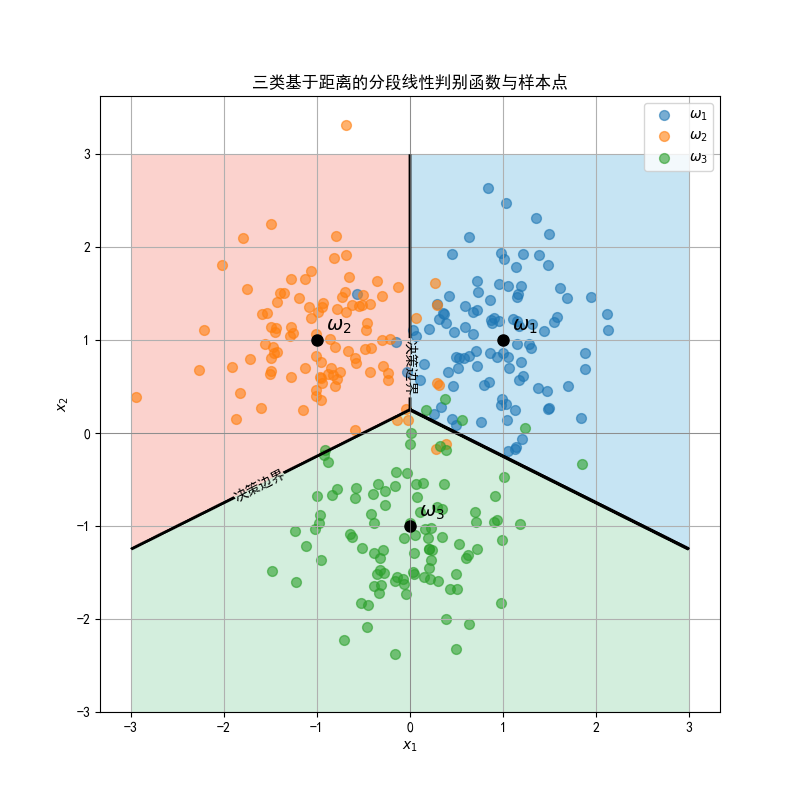
\includegraphics[scale=0.4]{T1分段分类.png}
    \caption{分段线性判别分类器}
    \label{fig:image1}
\end{figure}

\section*{第2题}
(1)非线性分类器包括多层感知机、径向基函数网络和循环神经网络。其中多层感知机和径向基函数网络属于前馈网络,循环神经网络属于反馈网络。

几种神经网络的工作原理:\\
(i)多层感知机:

多层感知机 (MLP) 是一种前馈神经网络,由输入层、隐藏层和输出层组成。每层由多个神经元构成,并且每个神经元与前一层的神经元相连接。MLP 的工作原理如下:

\begin{enumerate}
    \item 输入数据通过输入层传递到隐藏层。
    \item 每个隐藏层神经元对输入进行加权求和,并通过激活函数进行非线性变换。
    \item 最后一层输出层将经过隐藏层变换的信号进行加权求和并产生最终输出。
    \item 网络通过反向传播算法(Backpropagation)进行训练,调整网络中各层之间的权重,以减少输出误差。
\end{enumerate}
\[
\mathbf{y} = \sigma(\mathbf{W_2} \cdot \sigma(\mathbf{W_1} \cdot \mathbf{x} + \mathbf{b_1}) + \mathbf{b_2})
\]
其中,$\mathbf{x}$ 是输入,$\mathbf{W_1}$ 和 $\mathbf{W_2}$ 是权重矩阵,$\mathbf{b_1}$ 和 $\mathbf{b_2}$ 是偏置,$\sigma$ 是激活函数(如 Sigmoid、ReLU 等)。

(ii)径向基函数网络 (RBFN) 工作原理:\\
径向基函数网络(RBFN)是一种前馈神经网络,通常包含输入层、隐含层和输出层。RBFN 的工作原理如下:

\begin{enumerate}
    \item 输入数据传递到隐含层,其中隐含层的每个神经元使用径向基函数(通常是高斯函数)对输入进行变换。
    \item 计算输入点与每个隐含层神经元的距离,并通过该距离值对每个神经元的输出进行加权。
    \item 输出层使用加权求和的方式生成最终的输出。
    \item 网络通过最小化输出与目标之间的误差进行训练,更新权重。
\end{enumerate}

隐含层神经元的输出通常使用高斯径向基函数:
\[
\phi_i(\mathbf{x}) = \exp \left( -\frac{\|\mathbf{x} - \mathbf{c}_i\|^2}{2 \sigma_i^2} \right)
\]
其中,$\mathbf{c}_i$ 是隐含层第 $i$ 个神经元的中心,$\sigma_i$ 是该神经元的宽度,$\|\mathbf{x} - \mathbf{c}_i\|$ 是输入点与该中心的欧氏距离。

输出层则进行加权求和:
\[
\mathbf{y} = \sum_{i=1}^{N} w_i \phi_i(\mathbf{x})
\]
其中,$w_i$ 是每个隐含神经元的权重。

(iii)循环神经网络 (RNN) 工作原理:\\
循环神经网络(RNN)是一类能够处理序列数据的神经网络,其特点是网络中的节点之间存在反馈连接。RNN 的工作原理如下:

\begin{enumerate}
    \item 输入序列数据通过输入层传递到网络中,每个时间步的输入会影响当前时刻的状态。
    \item 网络的每个时间步都根据当前输入和上一个时间步的隐藏状态计算当前的隐藏状态。
    \item 每个时间步的输出不仅依赖于当前的输入,还依赖于前一时刻的状态。
    \item 网络通过反向传播算法(Backpropagation Through Time,BPTT)进行训练,以优化网络中的参数。
\end{enumerate}

RNN 的基本方程为:
\[
\mathbf{h}_t = \sigma(\mathbf{W_x} \cdot \mathbf{x}_t + \mathbf{W_h} \cdot \mathbf{h}_{t-1} + \mathbf{b})
\]
其中,$\mathbf{x}_t$ 是当前时间步的输入,$\mathbf{h}_t$ 是当前时间步的隐藏状态,$\mathbf{W_x}$ 和 $\mathbf{W_h}$ 分别是输入到隐藏层和隐藏层到隐藏层的权重矩阵,$\mathbf{b}$ 是偏置,$\sigma$ 是激活函数。

最终输出为:
\[
\mathbf{y}_t = \mathbf{W_y} \cdot \mathbf{h}_t + \mathbf{c}
\]
其中,$\mathbf{y}_t$ 是当前时间步的输出,$\mathbf{W_y}$ 是输出层的权重,$\mathbf{c}$ 是输出偏置。

(2)二层感知机(输入d维样本,隐层n个节点,输出c个节点)

(i)前向传播\\
step1.输入层到隐层的计算:\\
    输入样本 $\mathbf{x} \in \mathbb{R}^d$ 通过输入层传递到隐层。假设隐层的权重矩阵为 $\mathbf{W_1} \in \mathbb{R}^{n \times d}$,偏置为 $\mathbf{b_1} \in \mathbb{R}^n$,则隐层的输入为:
    \[
    \mathbf{z_1} = \mathbf{W_1} \mathbf{x} + \mathbf{b_1}
    \]
    隐层的激活输出为:
    \[
    \mathbf{a_1} = \sigma(\mathbf{z_1})
    \]
    其中,$\sigma(\cdot)$ 是激活函数(如 ReLU、Sigmoid 或 Tanh)。\\
step2.隐层到输出层的计算:\\
    隐层的输出 $\mathbf{a_1} \in \mathbb{R}^n$ 通过隐层与输出层之间的权重矩阵 $\mathbf{W_2} \in \mathbb{R}^{c \times n}$ 和偏置 $\mathbf{b_2} \in \mathbb{R}^c$ 计算输出层的输入:
    \[
    \mathbf{z_2} = \mathbf{W_2} \mathbf{a_1} + \mathbf{b_2}
    \]
    输出层的激活输出为:
    \[
    \mathbf{a_2} = \hat{\mathbf{y}} = \sigma(\mathbf{z_2})
    \]
    其中,$\hat{\mathbf{y}}$ 是网络的预测输出,$\sigma(\cdot)$ 是输出层的激活函数(通常是 softmax 或 sigmoid,取决于具体任务)。

(ii)损失函数使用平方误差(MSE)来衡量预测值 $\hat{\mathbf{y}}$ 和目标值 $\mathbf{y}$ 之间的差异:
\[
L = \frac{1}{2} \sum_{i=1}^{c} (\hat{y}_i - y_i)^2
\]
其中,$\hat{y}_i$ 是输出层的第 $i$ 个神经元的输出,$y_i$ 是目标标签的第 $i$ 个元素,$c$ 是输出层的维度。

反向传播算法通过计算损失函数相对于每个参数(权重和偏置)的梯度,然后通过梯度下降法更新网络的参数。

1. 计算输出层的误差:\\
    输出层的误差(梯度)为损失函数对输出层激活输出的导数:
    \[
    \delta_2 = \frac{\partial L}{\partial \hat{\mathbf{y}}} = \hat{\mathbf{y}} - \mathbf{y}
    \]
    其中,$\hat{\mathbf{y}}$ 是输出层的预测输出,$\mathbf{y}$ 是目标输出。

2. 计算输出层权重和偏置的梯度:\\
    输出层权重的梯度为:
    \[
    \frac{\partial L}{\partial \mathbf{W_2}} = \delta_2 \mathbf{a_1}^T
    \]
    输出层偏置的梯度为:
    \[
    \frac{\partial L}{\partial \mathbf{b_2}} = \delta_2
    \]

3. 计算隐层的误差:
    隐层的误差通过输出层的误差和权重矩阵 $\mathbf{W_2}$ 反向传播计算得到:
    \[
    \delta_1 = (\mathbf{W_2}^T \delta_2) \circ \sigma'(\mathbf{z_1})
    \]
    其中,$\circ$ 表示逐元素乘法,$\sigma'(\mathbf{z_1})$ 是激活函数的导数。

4. 计算隐层权重和偏置的梯度:
    隐层权重的梯度为:
    \[
    \frac{\partial L}{\partial \mathbf{W_1}} = \delta_1 \mathbf{x}^T
    \]
    隐层偏置的梯度为:
    \[
    \frac{\partial L}{\partial \mathbf{b_1}} = \delta_1
    \]

5. 参数更新:
    使用梯度下降法更新权重和偏置。设学习率为 $\eta$,则:
    输出层权重更新公式:
    \[
    \mathbf{W_2} \leftarrow \mathbf{W_2} - \eta \frac{\partial L}{\partial \mathbf{W_2}}
    \]
    输出层偏置更新公式:
    \[
    \mathbf{b_2} \leftarrow \mathbf{b_2} - \eta \frac{\partial L}{\partial \mathbf{b_2}}
    \]
    隐层权重更新公式:
    \[
    \mathbf{W_1} \leftarrow \mathbf{W_1} - \eta \frac{\partial L}{\partial \mathbf{W_1}}
    \]
    隐层偏置更新公式:
    \[
    \mathbf{b_1} \leftarrow \mathbf{b_1} - \eta \frac{\partial L}{\partial \mathbf{b_1}}
    \]
\section*{第3题}
(1)样本点:
\begin{center}
    \includegraphics[width=0.3\textwidth]{T3两类样本图.png}
    \captionof{figure}{两类样本点图}
    \label{fig:image2}
\end{center}

(2)二层感知机:

采用交叉熵为损失函数,经过超参数调试,发现:当隐层节点数量为10,初始学习率为0.1,并遂训练过程以固定步长衰减时,模型对训练数据的精度可以达到1。下面是损失函数曲线和精度曲线:
\begin{center}
    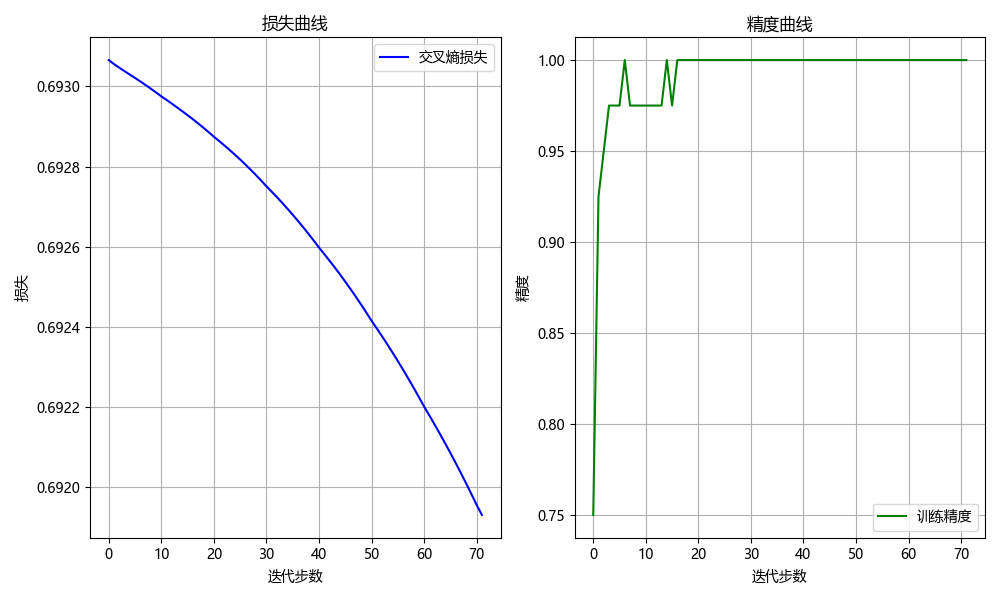
\includegraphics[width=0.6\textwidth]{T3(2)二层感知机.png}
    \captionof{figure}{损失函数及训练精度曲线}
    \label{fig:image3}
\end{center}

下面是决策面的绘制结果:
\begin{center}
    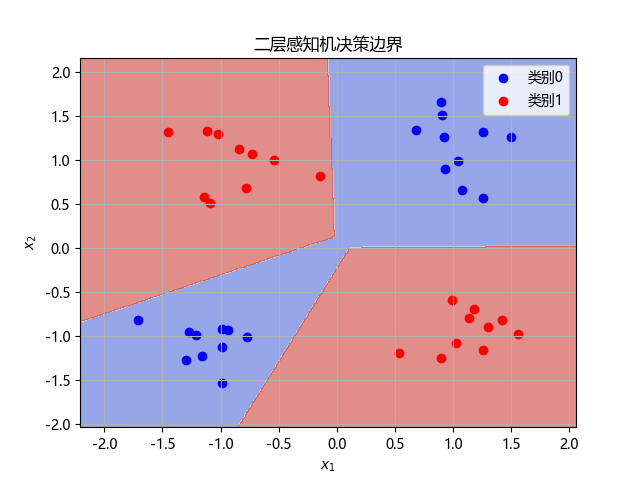
\includegraphics[width=0.6\textwidth]{T3(2)的决策边界.png}
    \captionof{figure}{(2)决策边界}
    \label{fig:image4}
\end{center}
(3)扩展多项式判别函数的Logistic回归:

下面分别绘制了损失函数(二值交叉熵)、训练精度:
\begin{center}
    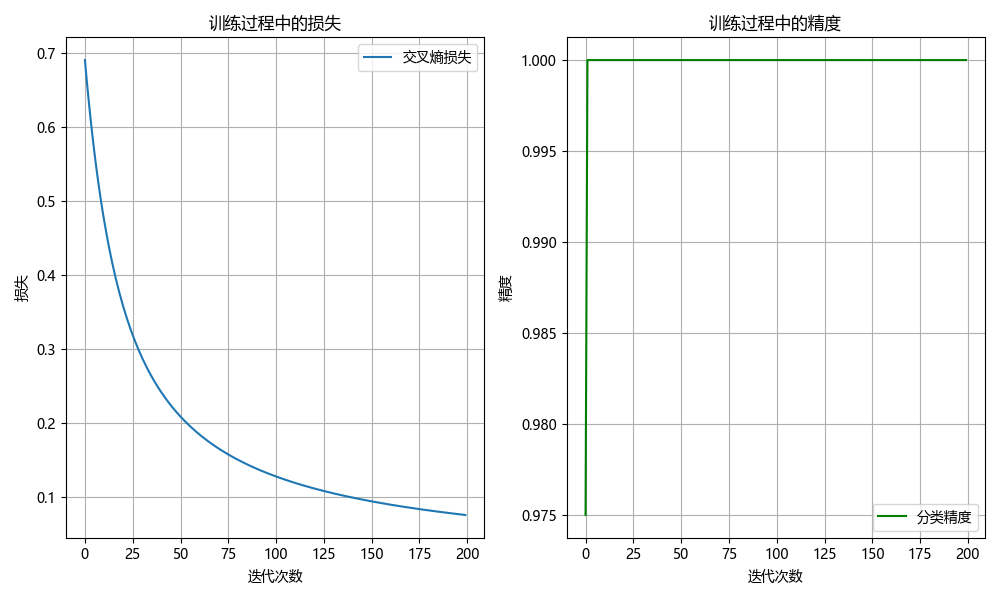
\includegraphics[width=0.6\textwidth]{T3(3)多项式logistic回归.png}
    \captionof{figure}{(3)损失函数和训练精度}
    \label{fig:image5}
\end{center}

下图为(3)的决策边界
\begin{center}
    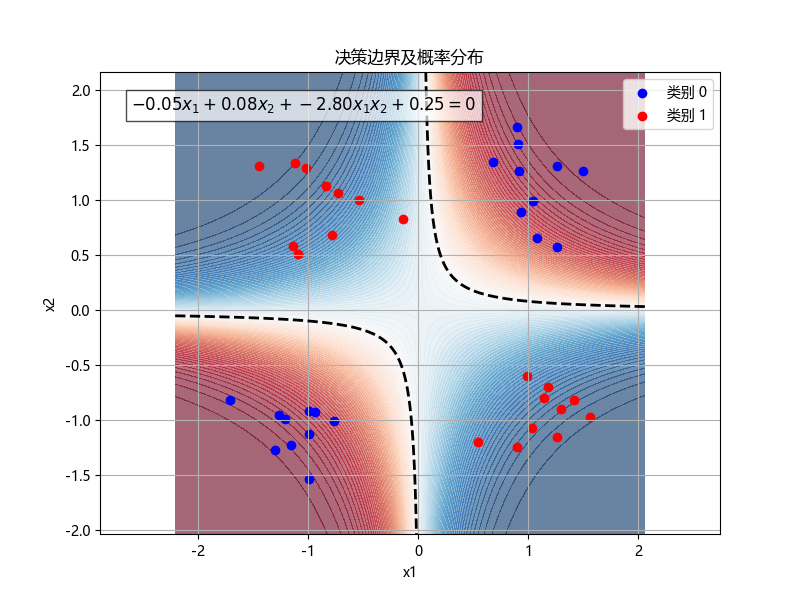
\includegraphics[width=0.6\textwidth]{T3(3)的决策边界.png}
    \captionof{figure}{(3)决策边界}
    \label{fig:image6}
\end{center}

\section*{第4题}

二层感知机网络结构:

第0层(输入层):输入向量$x\in \mathcal{R}^{256}$

第1层(隐层):

权重矩阵 $W_{1} \in \mathcal{R}^{256 \times H}$, $H$ 为 hidden\_size 的大小,偏置$b\in\mathcal{R}^{H}$,激活函数用ReLU函数。即\[ \hat{z_1}=ReLU(xW_1+b_1)\]

第2层(输出层);

权重矩阵 $W_{2} \in \mathcal{R}^{H \times 10}$, 偏置$b\in\mathcal{R}^{10}$,激活函数用softmax函数。即\[\hat{y}=softmax(z_1W_2+b_2)\]

损失函数:使用交叉熵损失\[L=-\frac{1}{N}\sum_{i=1}^{N}\sum_{j=1}^{10}y_{ij}log(\hat{y_{ij}})\]其中$y_{ij}$为真实标签,$\hat{y}$为预测概率

梯度下降法更新权重:

train()方法每轮前向传播一次,计算梯度,更新权重参数。
每一轮记录:\\
训练损失loss,训练精度 acc,测试错误率 test\_err = 1 - test\_acc

主要超参数为隐层神经元数量$hidden_size$和学习率$learning_rate$。

其中隐层神经元数量控制模型的“容量”,即模型学习复杂度,适当提升可以增强模型的表达力,但过大时会导致过拟合。实验发现,分别选取隐层神经元数量为64,256,512,1024,发现512时效果最好,继续增大后训练精度和测试精度无明显变化。

PS:2的幂次方与计算优化

(i)硬件对齐:现代计算硬件(如GPU)的内存分配和矩阵运算通常对2的幂次方(如256、512、1024)更友好。这些数值的内存对齐和并行计算效率更高,能加速训练。

(ii)并行化加速:神经网络中的矩阵乘法(如 W1 @ X)在2的幂次维度下,GPU的线程块调度更高效,减少资源浪费。


学习率$learning_rate$控制梯度下降中每次权重更新的步长,过小模型收敛慢,过大使得损失函数振荡或不收敛。多次实验发现,设置为0.002到0.004之间效果都不错。
最终取$hidden_size=512,learning_rate=0.003$,作出损失函数和(训练精度\&测试错误率)曲线如下:

\begin{center}
    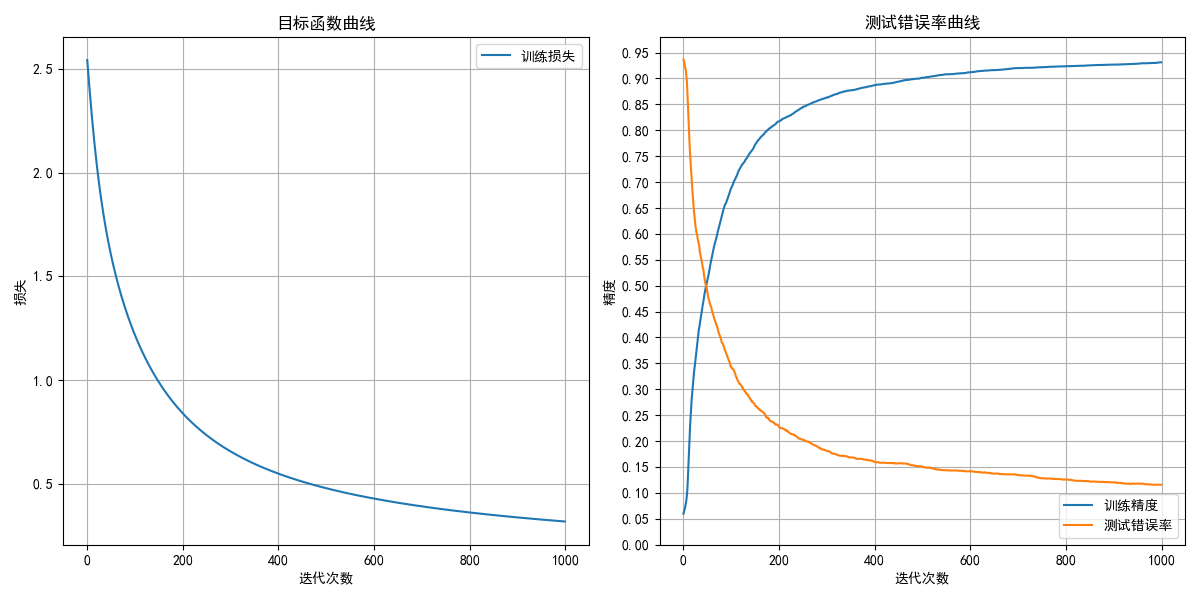
\includegraphics[width=0.6\textwidth]{0.93_0.12.png}
    \captionof{figure}{损失函数、训练精度、测试错误率随训练时间变化曲线}
    \label{fig:image7}
\end{center}
最终损失函数收敛到0.2左右,训练精度收敛到93\%左右,测试错误率控制在12\%以下。

\end{document}
